\chapter{Proposed implementation}\label{chap:proposal}
In this chapter, we are going to describe the implementation we propose, the technologies we intend to use and the models we aim to examine.


\section{Technologies}
In this thesis, we implement all of the studied models in python deep learning library Keras with Tensorflow backend. All of the experiments are conducted on NVIDIA GTX 1070.

% ...Software, frameworks, libraries to be used... GPU used
\section{Benchmark datasets}

In this section, we are going to describe the datasets which will be used for the evaluation purposes of this thesis. All of the datasets mentioned below were made publicly available for research purposes.
\subsection{ITOP}
The Invariant-Top View Dataset (ITOP) \cite{haque2016viewpoint} consists of approximately 50k real-world depth images from two camera viewpoints (front view and top view). It captures 20 people, each performing 15 different actions. The dataset comes with the initial partition of the data into the train and test set. The labeled train and test data contain around 18k and 5k samples from each viewpoint, respectively. Besides the depth images and the ground truth joint labels, the dataset also includes raw point clouds. The skeletal model in this dataset is described by 15 body joints. Sample depth maps from the dataset are shown in Figure \ref{fig:itop}. As can be seen in the figure, the depth images are rather noisy, but the noise can be partly reduced by several background segmentation methods.\par

\vspace{5mm}
\begin{figure}[H]
\begin{center}
  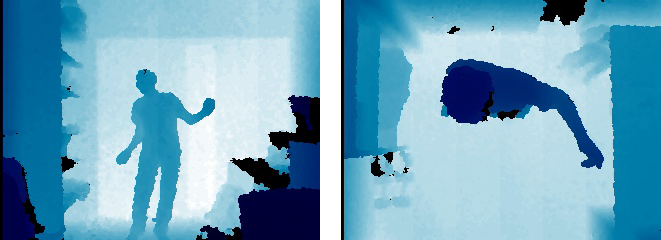
\includegraphics[height=130px]{images/implementation/itop.png}
  \caption[Sample depth images from the ITOP dataset \cite{haque2016viewpoint}.]{Sample depth images from the ITOP dataset \cite{haque2016viewpoint} (front and top view).}
  \label{fig:itop}
\end{center}
\end{figure}

\noindent
The current state-of-the-art on ITOP dataset was claimed in \cite{Marin18jvcir}, where the 100\% accuracy at 10cm precision was reached, which means every joint was predicted within 10cm from its ground truth position. In the paper, they also claim to have reached the mean error of approximately 0.9cm on ITOP dataset (0.19cm on the front-view data), which is the best result achieved on the stated dataset, up to our knowledge.

\subsection{UBC3V}

The UBC3V \cite{Shafaei16} is a synthetic dataset made for the task of pose estimation from multiple cameras. It contains around 6 million synthetic depth frames structured in three parts according to the complexity of the human postures – easy, medium and hard pose. The pose in each frame is represented by the position of 18 skeletal joints. It captures a total of 16 characters and each frame is observed from three different viewpoints. Therefore, the samples can be treated both as multi-view (point clouds from three cameras merged into one), or single-view postures (each sample handled separately). Although the multi-view point clouds describe a particular posture in a more complex way, considering the use-case in most of the real-time applications, the single-view samples are often the preferred option, due to the difficulty of the task of multiple camera synchronization.\par

\vspace{5mm}
\begin{figure}[H]
\begin{center}
  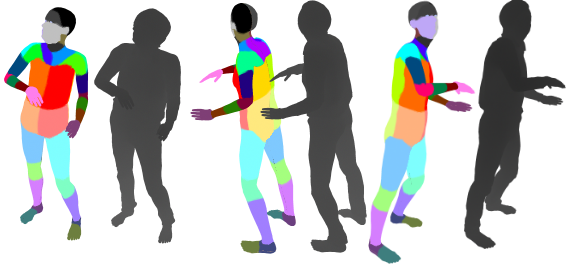
\includegraphics[height=130px]{images/implementation/ubc3v.png}
  \caption[Sample data from the UBC3V dataset \cite{Shafaei16}.]{Sample data from the UBC3V dataset (the figure shows the same pose from three different cameras) \cite{Shafaei16}.}
  \label{fig:ubc3v}
\end{center}
\end{figure}

\noindent
 The depth data are available in the form of depth images, but can be converted into point clouds in world reference coordinates using the intrinsic and extrinsic camera parameters. The ground truth labels are composed of 18 joints per posture, and the dataset also comprises a segmentation of each point cloud into 43 body regions (as can be seen in Figure \ref{fig:ubc3v}).

\subsection{MHAD}
The Berkeley Multimodal Human Action Database (MHAD) \cite{Vidal:2013:BMC:2478277.2478412} was recorded on real humans. It contains 11 actions performed by 7 male and 5 female subjects. Each subject performed each of the actions 5 times, which yields about 660 action sequences corresponding to about 82 minutes of total recording time. The total number of depth frames is over 250k. The skeleton structure in this dataset is defined by 35 joint locations (as shown in Figure \ref{fig:mhad_skeleton}). Two of the performed actions involve a chair, used for the subject to sit down and stand up. It is worth a mention, that the chair itself provides a lot of clutter in the depth data.\par

\vspace{5mm}
\begin{figure}[H]
\begin{center}
  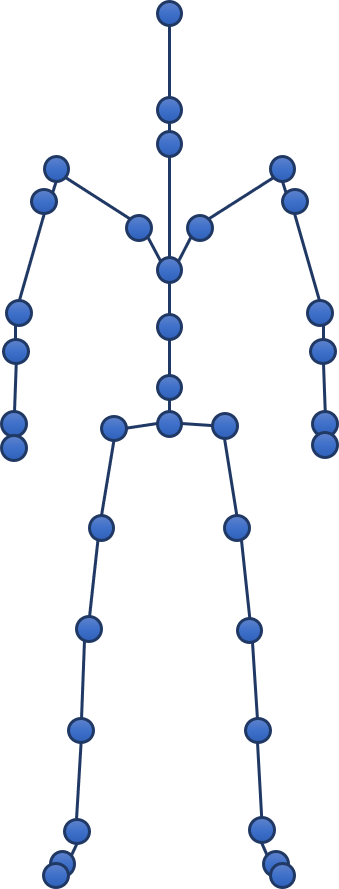
\includegraphics[height=130px]{images/implementation/mhad_skeleton.png}
  \caption[The body skeleton structure used in MHAD dataset \cite{Vidal:2013:BMC:2478277.2478412}.]{The body skeleton structure used in MHAD dataset \cite{Vidal:2013:BMC:2478277.2478412}, described by 35 joint location coordinates.}
  \label{fig:mhad_skeleton}
\end{center}
\end{figure}

\noindent The whole dataset was captured by multiple devices, including cameras, depth sensors, accelerometers and microphones. Two kinect cameras were used and synchronized to acquire the depth data, one placed in front of the subject, the other one at the back. Intrinsic and extrinsic camera parameters are provided to extract the scene as a point cloud with real-world coordinates.\par

\subsection{CMU Panoptic Dataset}

The CMU Panoptic \cite{Joo_2017_TPAMI} is a massive multi-view dataset containing video recordings from 480 VGA cameras and more than 30 HD cameras, RGB and depth data from 10 Kinect v2 sensors and 3D body poses. The facial and hand keypoint data is available as well. The skeleton representation including the face and hands consists of 19 body joints. The full dataset yields around 6 hours of recordings. The synchronization of the devices is hardware-based, although, as the authors state in the database description, there is no way to perfectly synchronize multiple Kinects. However, most of the data is aligned accurately by hardware modifications for time-stamping. The calibration parameters are provided for all the cameras, therefore 3D point clouds in real world coordinates can be easily generated. The multi-view point clouds are created by merging single-view data from the multiple Kinects captured within a time interval of ca. 15 milliseconds. If the human motion is fast, there exist certain misalignments, but they can be further filtered according to the delivered synchronization tables, in order to leave out the misaligned frames.\par
\vspace{5mm}
\noindent
During our study, we utilize only certain parts of the CMU Panoptic dataset, since we are strictly concentrating our research on a single person pose estimation, while the CMU data also contain sequences capturing multiple people in a single frame. Aside from that, for some of the sequences, only certain types of data are included. Specifically, we use the 'range of motion' section of the database, since it is the only section restricted to a single actor at a time, which involves the ground truth 3D poses. Also, we construct the 3D point clouds from only 3 out of 10 Kinect cameras, as the complete set of depth sensors generate extremely dense data, which is not likely obtainable with common setup. Besides, the three Kinects capture the scene within an angular range large enough to yield a full 3D body pose. Since we are not focusing on face keypoints and detailed hand pose estimation, we exclude the corresponding joints from the skeleton structure, what leaves us with a set of 15 body joints.\par
\vspace{5mm}
\noindent The database captures multiple actors of different gender, age and body shape. Given the fact the dataset has been recorded in a special environment of the Panoptic studio, the amount of noise in the scene is very limited. However, the surrounding walls and the floor still need to be removed in the pre-processing stage. The CMU Panoptic dataset does not come with any train and test split, so for the sake of our experiments, we established the test set as random 20\% of the data. From the remaining train samples, another 20\% are used as a validation set.


%\subsection{Novel dataset} 
\section{Approaches}
The goal of our study is to implement several different approaches to the task of human pose estimation using neural networks. Among the methods we implement are both existing state-of-the-art neural models, as well as our novel approach we propose in this thesis – a two-stage pipeline called Four-channel Pose Estimation. We present the existing models we re-implement, and our novel approach in the subsequent sections.

\subsection{Deep Depth Pose model}
One of the aims of this work, is to implement the Deep Depth Pose model (DDP) \cite{Marin18jvcir} in Keras framework. We consider this an essential step to propose a state-of-the-art pose estimation model performing on depth data, since the DDP model claims to outperform all of the present methods on the examined datasets. Originally, the model is implemented in Matlab and while some parts of the code (mostly testing) are publicly available, the training procedures have not been published.\par
\vspace{5mm}
\noindent
The main idea behind the stated method is incorporating a set of predefined prototype human poses. The convolutional neural network outputs a vector containing weights, each corresponding to particular prototype pose. The weighted prototypes are then summed up producing the final estimated pose. The predefined prototype poses should ideally cover the largest possible range of human poses, so that by their linear combination we can obtain any desired pose during the testing. Hence, the set of prototype poses is formed by applying K-means clustering on the training dataset.

\subsection{Point-Based Pose Estimation model}

% TODO toto cele uz do proposed implementation, potom v implementation uz implementacne detaily, preprocessing dat, upravy modelu
The Point-Based Pose Estimation model (PBPE) \cite{Ali19} is an approach to 3D human pose estimation from depth data, remarkable by several of its attributes. The whole network consists of two branches, the regression branch and the auxiliary segmentation branch. The output of the model is a 3D body pose, given by the coordinates of skeletal joints. One of the benefits of the method is the possibility of omitting the auxiliary branch in the testing phase, where the model is already trained, and by this restriction of the model's depth and complexity, the computational cost and prediction time can be cut down.\par
\vspace{5mm}
\noindent Of great significance for our thesis is the fact, that the input to the PBPE network is directly in a form of an unstructured point cloud. This may be convenient for a number of reasons, one of them being the acquisition of a sparser representation of the human body pose, in comparison to commonly used depth maps. The more density the input covers, the more computations have to be performed in the network, therefore point clouds offer more effective data processing even in complex model architectures. The model architecture is inspired by PointNet model \cite{DBLP:journals/corr/QiSMG16}. Inside the PointNet as well as the PBPE model, the point clouds are processed using the pseudo-convolutions with kernel size $1 \times 1$, which are generally employed to change the filter space dimensionality, mostly reducing the number of depth channels.\par % TODO vysvetlit tu este blizsie 1x1 konvolucie ? radsej tu nez v implementation
\vspace{5mm}
\noindent Since the source code for the PBPE model has not been made public prior to working on this study, we aim to implement the model in Keras framework from scratch and evaluate the results on benchmark datasets.

\subsection{Four-channel Pose Estimation}

An important part of our work is to develop a novel method for human pose estimation. We introduce the Four-channel Pose Estimation – a two-stage pipeline, which takes a point cloud as an input, and outputs the 3D coordinates of the estimated skeletal joint positions. Retaining the idea of handling point clouds directly with pseudo-convolutions, first stage of the pipeline is based on a segmentation network, which classifies the points representing a human pose into the corresponding body regions. In the second stage, the input point cloud containing the point coordinates is concatenated with the output regions from the segmentation network, thus forming a four-channel point cloud input. Such produced data, conserving together the local as well as the global information, is then fed into the second model – the regression network, where the joint coordinates are finally regressed. Both networks make use of residual connections added to the shared multilayer perceptron blocks, to strengthen the feature propagation. \par
\vspace{5mm}
\noindent Similarly to the models mentioned above, we implement our novel approach in Keras framework as well. To be able to compare the performance of our model to that of the existing ones, the same benchmark datasets are used for the evaluation.


%\begin{minipage}{\textwidth}
%	Sily v našom modeli možno rozdeliť do dvoch skupín:
%	\begin{itemize}
%		\item interné sily
%		\item externé sily
%	\end{itemize}
%\end{minipage}\newline




